\chapter{Experimental Evaluation} \label{sec:exev}
In this section, conducted experiments are explained, and newly introduced metrics evaluate performances of agents.

\section{Experiments}
The Atari environment ``MsPacmanNoFrameskip-v4'' with the \textit{tag} ``final'' and \textit{run number} ``1'' was used for the experiments. The experiments are performed by agents trained with the algorithms from section \ref{sec:ai_agents}. \citeA{2018arXiv181207069P} provides previously trained \textit{frozen} models of the agents in a GitHub repository\footnote{\url{https://github.com/uber-research/atari-model-zoo}}, as well as source code, to test those agents. The source code was adjusted, so that information about how rewards are achieved could be accessed. This was done by counting how often certain rewards, see section \ref{ssec:pacman}, was gained. A total of five experiments were performed. The results are taken from the respective averages of over 30 episodes. 

\paragraph{First experiment}
In the first experiment, samples of the rewards and \textit{non-rewards}, the number of rewards with zero value, were collected, until an episode finishes, which was caused by losing all lives. This experiment's objective was to measure the agents' efficiency by counting the number of non-rewards and compare their values. An agent gains a non-reward each time it walks on an empty field.

\begin{table}[H]
	\caption[Average achieved results in 30 episodes]{Average achieved results from agents across 30 episodes}
	\centering
	\scalebox{0.7}{\begin{tabular}{l*{4}{c}} 
		\hline \\ 
		Algorithm&Rewards&Non-Rewards&Frames   \\  [2ex] 
		\hline \\
		A2C & 862 & 693 & 751 \\ [2ex]
		Ape-X & 8035 & 2126 & 2601\\ [2ex]
		DQN & 4180 & 1481 & 1791 \\ [2ex]
		ES & 1683 & 601 & 659\\[2ex]
		GA & 290 & 486 & 513 \\ [2ex]
		Rainbow & 2370 & 697 & 851\\ [2ex]
		\hline
	\end{tabular}}
	\label{tab:eva1}
\end{table} 
However, as seen in Table \ref{tab:eva1}, a high non-reward count is guaranteed, by just playing the game long enough.

\paragraph{Second experiment}
In the second experiment other details, such as the number of pellets, power pellets, fruits, ghosts and ghosts successive, were counted. This made clear how the reward for each agent is accumulated. With these new results, the method from \ref{ssec:sc2le} is applicable, where a complex task is divided into simpler sub-tasks, i.e. eating pellets, fruits and ghosts. The full results are shown in Table \ref{tab:eva2}.
\begin{figure}[H]
	\centering
	\subfloat[Ghosts x2]{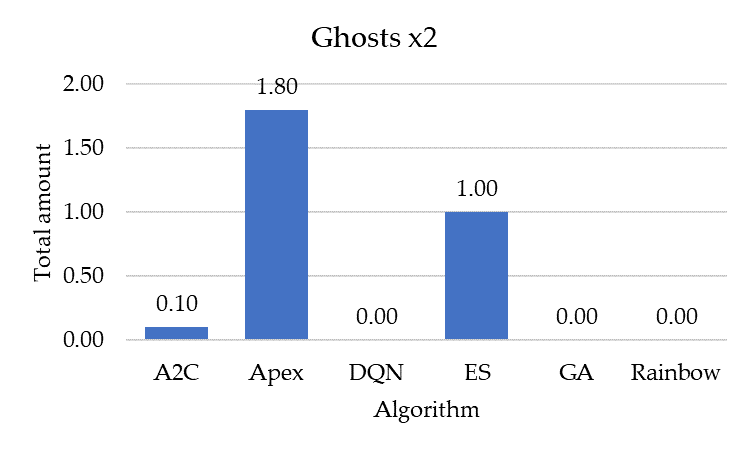
\includegraphics[scale=.52]{source/images/eval/ad_ghost2} }
	\smallskip
	\subfloat[Ghosts x3]{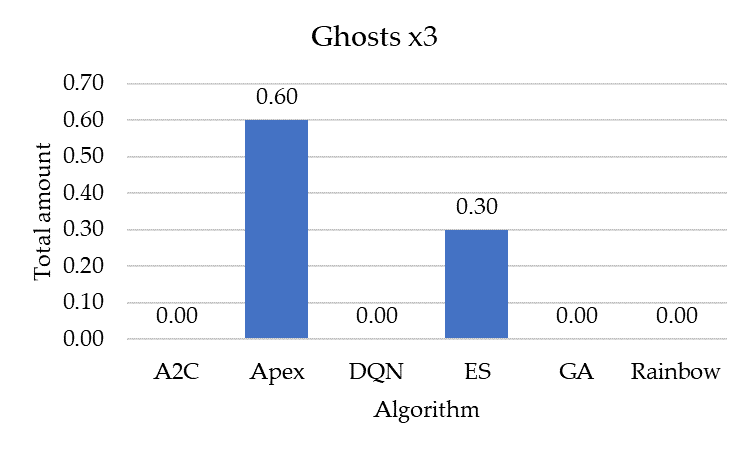
\includegraphics[scale=.52]{source/images/eval/ad_ghost3} } 
	\qquad
	\subfloat[Fruits]{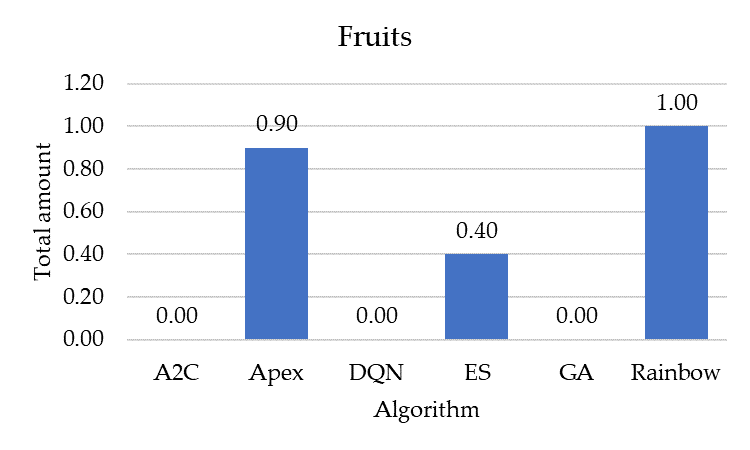
\includegraphics[scale=.52]{source/images/eval/ad_fruits} }
	\caption[Performance in sub-tasks]{Performance of the agents in relation to the sub-tasks across 30 episodes. (a) and (b) display the number of successive eaten ghosts, 2 and 3, respectively. }
	\label{fig:ex2}
\end{figure}

Previously, the \nameref{ssec:apex} and \nameref{ssec:dqn} agents were placed first and second, respectively. However, by rating the agents relative to the sub-tasks, the ranking changed, as seen in Figure \ref{fig:ex2}.The \nameref{ssec:rain} agent performs best at eating fruits, followed by the Ape-X and \nameref{ssec:es} agent. The remaining agents do not eat fruits at all. The ranking does not change for the pellet- and ghost-task, but it does for the number of successive ghosts. It changes in favor of the ES and \nameref{ssec:a2c} agent. Both outperform the others, except the Ape-X agent. 

However, the results for this experiment are not 100\% accurate, because as previously mentioned, the reward for eating a single ghost is 100. It is still the same for eating a fruit in the second level. Regularly, the Ape-X and DQN agents are proceeding to the second level. This is observed by counting the number of power pellets, since every level has exactly four of them. In the case of an agent gaining 100 points, it is accounted for by the ghosts' number. Therefore, the number of fruits is ignored for the second level. To avoid this issue and evaluate the agents uniformly, a third experiment is conducted.

\paragraph{Third experiment}
In the third experiment the agents play only the first level. This is accomplished by terminating the episodes, when all pellets are eaten. In this experiment, the overall ranking changed. The Rainbow agent accumulates the most rewards, by outperforming the other agents in the fruits- and ghosts-task, as seen in Figure \ref{fig:ex3}.

\begin{figure}[H]
	\centering
	\subfloat[Pellets]{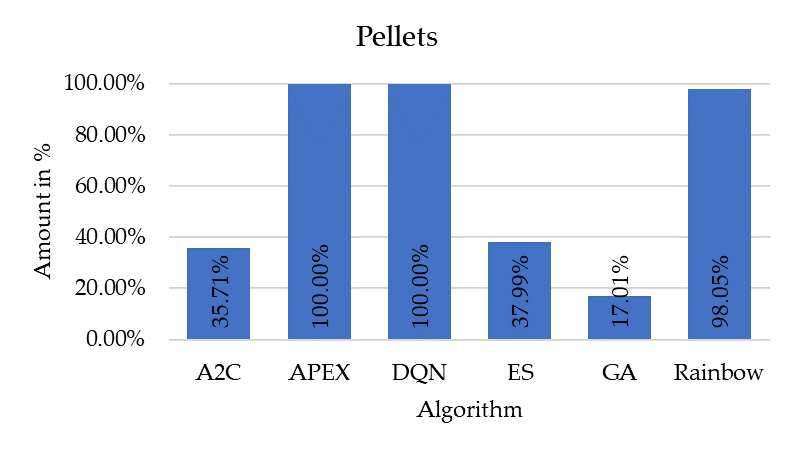
\includegraphics[width=6.5cm, height=4.25cm]{source/images/eval/pro_pel} }
	\smallskip
	\subfloat[Fruits]{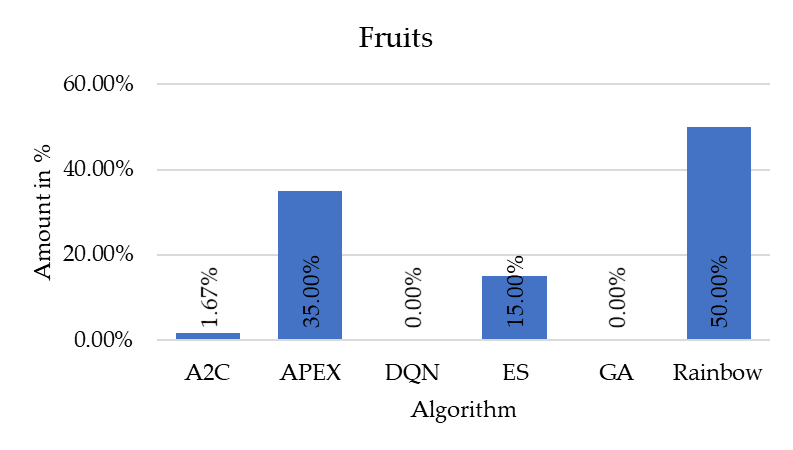
\includegraphics[width=6.5cm, height=4.25cm]{source/images/eval/pro_fruits} } 
	\qquad
	\subfloat[Ghosts]{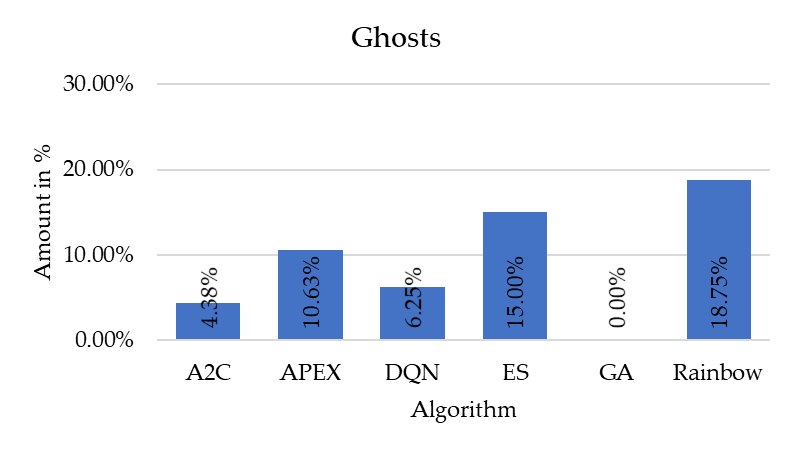
\includegraphics[width=6.5cm, height=4.25cm]{source/images/eval/pro_ghosts} }
	\caption[Performance in sub-tasks in level 1]{Performance of the agents in relation to the sub-tasks across 30 episodes in the first level. (a), (b) and (c) shows the percentage of eaten pellets, fruits and ghosts, respectively.}
	\label{fig:ex3}
\end{figure}
The result in the pellet-task is expected for the Ape-X, and DQN agents since both of them can clear the first level. The rainbow agent barely fails to pass the first level, by missing three pellets, as shown in Table \ref{tab:eva3}.

\paragraph{Fourth experiment}
For the fourth experiment the agents performed a random action with a 5\% probability in level one. The reason for this is to see how the agents manage the exploration-exploitation trade-off \cite{thrun1992role}. The value for the probability is taken from \cite{2013arXiv1312.5602M}. Generally, all agents improved in terms of total reward, as seen in Table \ref{tab:eva5}. The ranking changed for the upper part of the list, with the DQN agent being first, followed by the Rainbow and the Ape-X agent, in terms of total reward. The Ape-X and DQN agent have less lives. On the contrary, the Rainbow agent manages to collect all pellets and clear level one. The ranking for each sub-task changes as well, as seen in Figure \ref{fig:ex5}.

\begin{figure}[H]
	\centering
	\subfloat[Pellets]{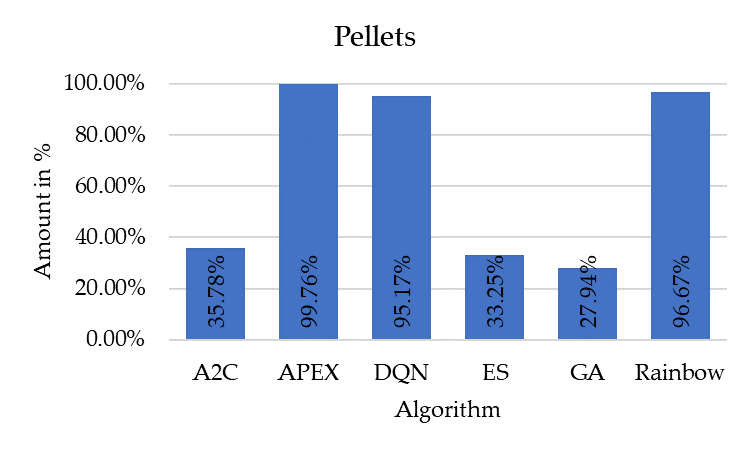
\includegraphics[width=6.5cm, height=4.25cm]{source/images/eval/rand_pel} }
	\smallskip
	\subfloat[Fruits]{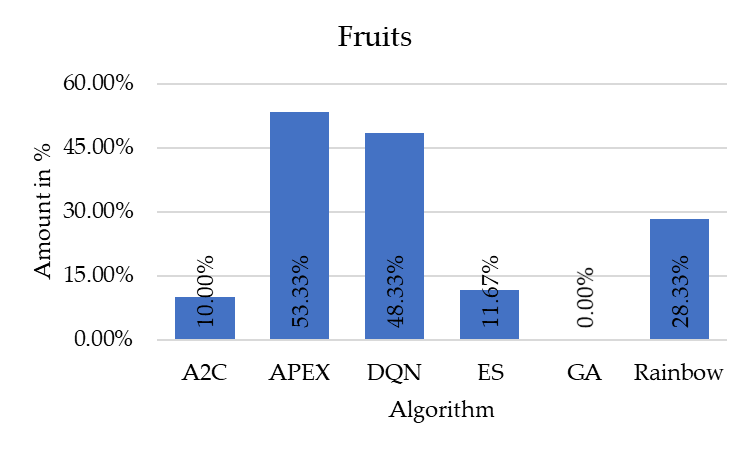
\includegraphics[width=6.5cm, height=4.25cm]{source/images/eval/rand_fruits} } 
	\qquad
	\subfloat[Ghosts]{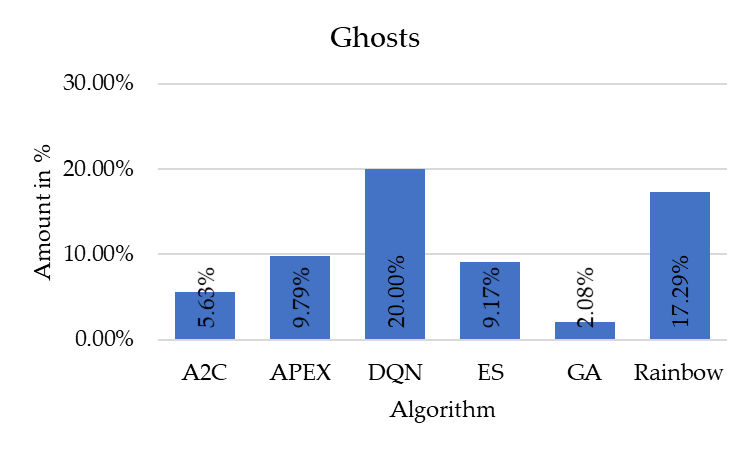
\includegraphics[width=6.5cm, height=4.25cm]{source/images/eval/rand_ghosts} }
	\caption[Performance in sub-tasks with 5\% random action probability]{Performance of the agents in relation to the sub-tasks across 30 episodes in the first level with 5\% random action probability.}
	\label{fig:ex5}
\end{figure}

\paragraph{Fifth experiment}
The fifth experiment is about the performance in the second level of the game. The DQN agent outperforms the Ape-X in all sub-tasks, except the fruit-task, as seen in \ref{tab:eva4}. In the fruit-task, both agents have zero, because fruits are not counted. However, the Ape-X agent still outperforms the DQN, in terms of total rewards, by eating ghosts successively.

\begin{table}[H]
	\caption[Average achieved results in the second level across 30 episodes] {Average achieved results in the second level across 30 episodes}
	\centering
	\scalebox{0.7}{\begin{tabular}{l*{6}{c}} 
		\hline \\ 
		Algorithm&Lives&Rewards&\%-Pellets&\%-Fruits&\%-Ghosts&Ghosts x2   \\  [2ex] 
		\hline \\
		APEX & 0.87 & 2581.33 & 98.35 & 0 & 16.67 & 0.93 \\ [2ex]
		DQN & 0 & 2280.00 & 98.70 & 0 & 18.75 & 0\\ [2ex]
		\hline
	\end{tabular}}
	\label{tab:eva4}
\end{table} 
Frequently, the Ape-X passes the second level, which explains the results in Table \ref{tab:eva1}.

\section{Evaluation}
The evaluation of the agents is based on the following metrics, performance in the sub-tasks, efficient pathing and an action-related metric. The data set from the third experiment is used for the evaluation, due to uniformity. 

\subsection{Performance sub-tasks}
There are three sub-tasks: pellet-, fruit- and ghost-task. The performance of an agent is measured by weighting those tasks. By observing results from the previous experiments, it is noticeable that some agents focus more on eating ghosts and other agents more on eating pellets. Agents eating pellets maximize their score by clearing the level and agents eating ghosts maximize their score by eating ghosts successively. Therefore, three evaluations are conducted in regards to playstyle. These are \textit{neutral}, \textit{passive} and \textit{aggressive}. All playstyles are weighted differently.

\paragraph{Neutral}
In the first evaluation, all sub-tasks are weighted equally, meaning around 33\%. The results are illustrated in Figure \ref{fig:sub_neu} and additional information can be seen in Table \ref{tab:eva7}. The Rainbow agent performs the best by reaching 56\% of the total score, closely followed by the Ape-X agent with 49\%. The GA and A2C agent did not perform so well; they reached only 6\% and 14\%, respectively. The DQN forms the center with 35\%.

\begin{figure}%
\centering
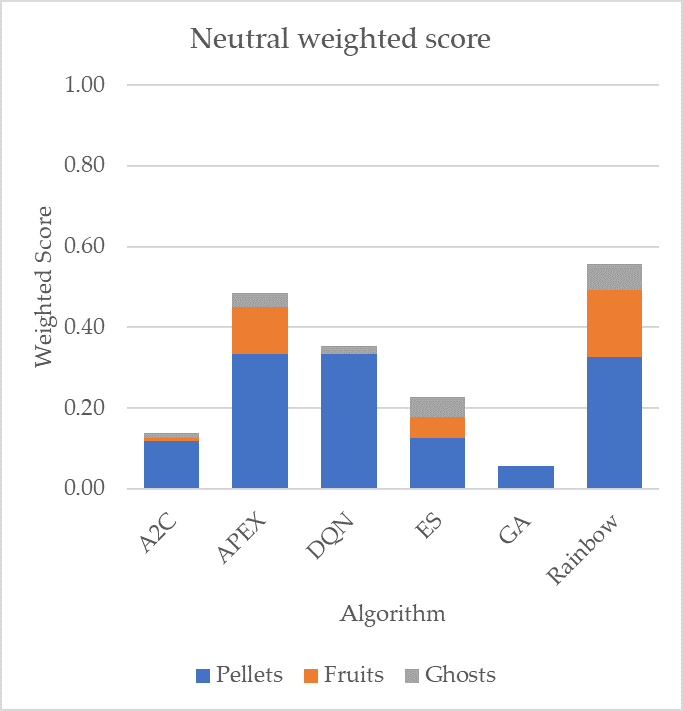
\includegraphics[scale=0.5]{source/images/eval/sub_neu}%
\caption[Illustration from the results of the neutral playstyle]{Illustration from the results of the neutral playstyle. Maximum possible score is 1 by combining the scores from each sub-task.}%
\label{fig:sub_neu}%
\end{figure} 

\paragraph{Passive}
The passive playstyle is safe. The focus is to clear the level by eating all pellets in order to maximize the total score. The weights for this playstyle are 60\% on the pellet-task and 20\% each for the fruit- and ghost-task. Detailed information can be seen in Table \ref{tab:eva9}. 
\begin{figure}[H]%
\centering
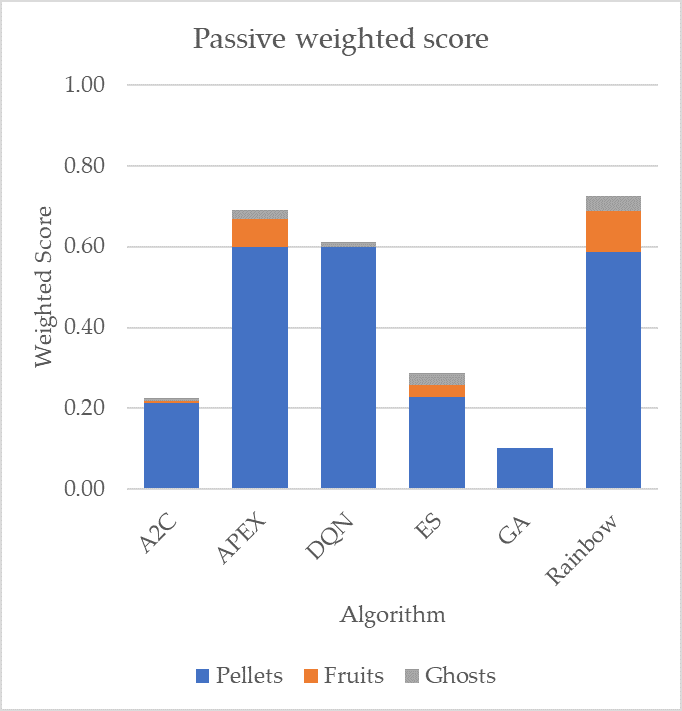
\includegraphics[scale=0.5]{source/images/eval/sub_pass}%
\caption[Illustration from the results of the passive playstyle]{Illustration from the results of the passive playstyle. Maximum possible score is 1 by combining the scores from each sub-task.}%
\label{fig:sub_pass}%
\end{figure}
By shifting the weights in favor of the pellet-task, all agents are generally performing better than with a neutral playstyle. The ranking order did not change, but the agents were able to close up, or further, the distance among them. DQN agent closed up its distance to the Ape-X agent from 14\% to 8\%, as well as from 21\% to 12\% compared to the Rainbow agent. The Rainbow agent was also able to widen its gap. Previously the difference was 50\% to the GA agent and in regards to the passive playstyle, it rose to 63\%. The results are illustrated in Figure \ref{fig:sub_pass}.

\paragraph{Aggressive}
The aggressive playstyle is risky, because the agent focuses on eating ghosts to maximize its score. The score for the ghost-task is weighted with 60\%, while the other sub-task are weighted with 20\% each. The results are illustrated in Figure \ref{fig:sub_agg} and further details can be seen in Table \ref{tab:eva10}.
\begin{figure}[H]%
\centering
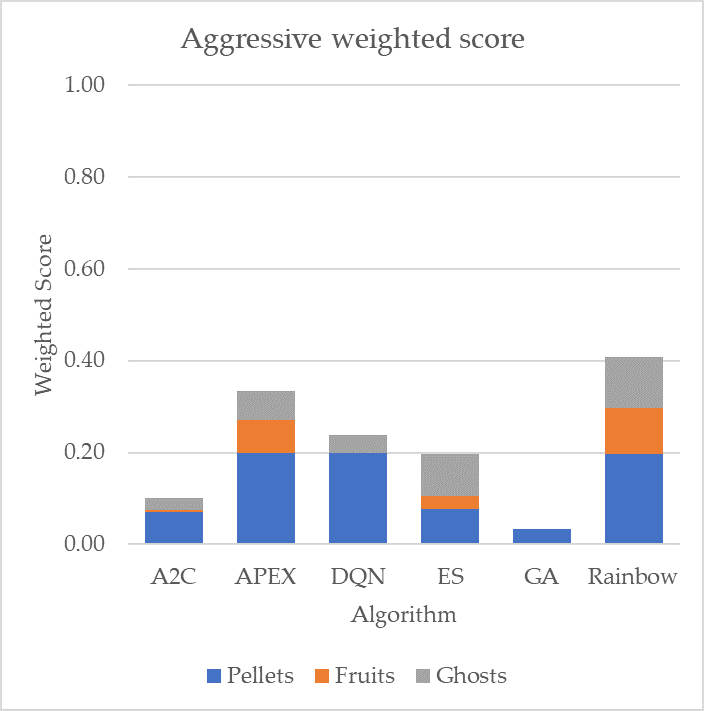
\includegraphics[scale=0.5]{source/images/eval/sub_agg}%
\caption[Illustration from the results of the aggressive playstyle]{Illustration from the results of the aggressive playstyle. Maximum possible score is 1 by combining the scores from each sub-task.}%
\label{fig:sub_agg}%
\end{figure}
The overall performance of the agents dropped because no agent was able to master this playstyle. To get 100\% in the ghost-task, the agents have to eat four ghosts with one power pellet, four times. This requires strategical planning and perfect execution\footnote{\url{https://www.youtube.com/watch?v=LnT8xPZw5jA}} and may cost efficiency. The overall ranking is the same as before, but again, the gap between agents changed with a different playstyle. None of the agents reaches half of the total score, with 41\% being the highest for the Rainbow agent. The gap between the best and worst-performing agents dropped from 63\% to 38\%. Compared to the previous results, the drop of the ES agent is not as big as the top three agents. This is reflected by the score gap between the ES agent and the Ape-X and DQN agents. In the passive playstyle, the difference was 38\% and 32\%, respectively. For the aggressive playstyle, it shrunk to 13\% and 4\%, respectively. The same goes for the A2C agent, the gap went from 46\% and 38\% to 23\% and 14\%, respectively.

\subsection{Efficiency}
Efficiency was measured by capping the episodes at 517 frames, which is the value of the agent with the lowest play-time. As seen in Table \ref{tab:eva6}, the Ape-X agent is the most efficient one, by having a reward to non-reward ratio of 4.57, followed by the DQN and Rainbow agent.
\begin{table}[H]
	\caption[Average results of agents in approximately 517 frames] {Average results of agents in approximately 517 frames}
	\centering
	\scalebox{0.7}{\begin{tabular}{l*{5}{c}} 
		\hline \\ 
		Algorithm&Lives&Rewards&Non-Rewards&Ratio  \\  [2ex] 
		\hline \\
		A2C & 1.47  & 543.67 & 476.20 & 1.14 \\ [2ex]
		APEX & 3.00 & 1800.33 & 394.23 & 4.57 \\ [2ex]
		DQN & 3.00 & 1573.67 & 394.90 & 3.98 \\ [2ex]
		ES & 1.50 & 1424.00 & 465.57 &  3.06\\ [2ex]
		GA & 0.53  & 295.33 & 478.27 &  0.62 \\ [2ex]
		Rainbow & 2.00  & 1537.67 & 414.63 & 3.71\\ [2ex]
		\hline
	\end{tabular}}
	\label{tab:eva6}
\end{table} 
Contrary to the other agents, the GA agent has a $<1$ ratio, which means that it gets more zero rewards than actual rewards. This makes the GA agent the most inefficient one. It is noticeable that the higher the number of lives of an agent, the more efficient it is. However, the gap between the ratio values of the A2C and ES agent compared to the other agents is too high to conclude that agents with more lives are more efficient.


\subsection{Actions}
The initial plan was to measure APM, but this does not work out because every agent had the same APM in this setup. Therefore, another approach was taken to measure the performance based on actions.
\begin{figure}[H]
	\centering
	\subfloat[GA]{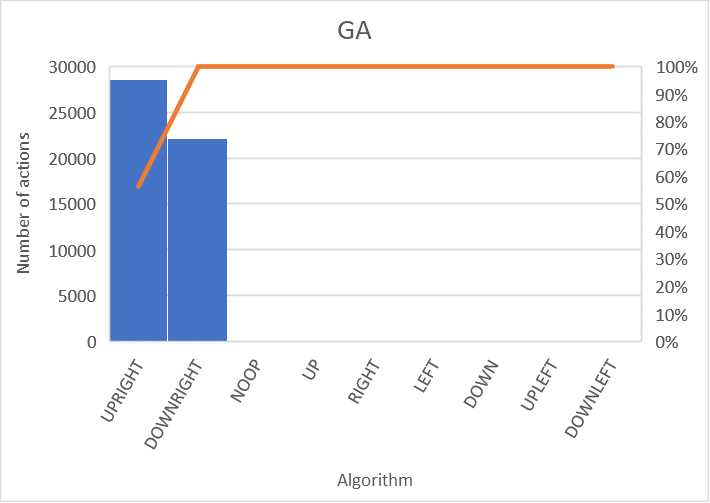
\includegraphics[scale=0.75]{source/images/eval/histo_ga} }%
	\qquad
	\subfloat[Rainbow]{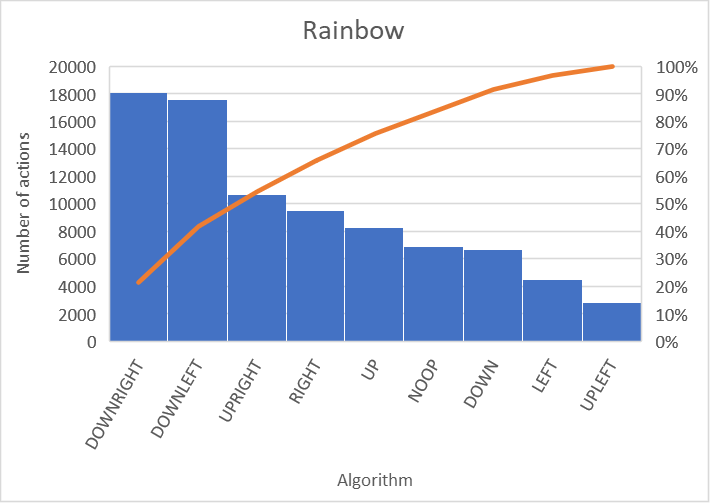
\includegraphics[scale=0.75]{source/images/eval/histo_rain} }%
	\caption[Action-distribution GA and Rainbow agent]{Action-distribution GA and Rainbow agent. The other agents' action-distributions are illustrated in Appendix \ref{app:aceva}, alongside with these two.}
	\label{fig:histo_ga_rain}
\end{figure}
For this evaluation, the number of each action was counted, as well as the number of changed actions. In accordance with previous experiments, the agents that performed a more extensive range of actions generally performed better, as illustrated in Figure \ref{fig:histo_ga_rain}. This also applies to higher numbers of changed actions, as seen in Figure \ref{fig:ac_changed}.
\begin{figure}[H]%
\centering
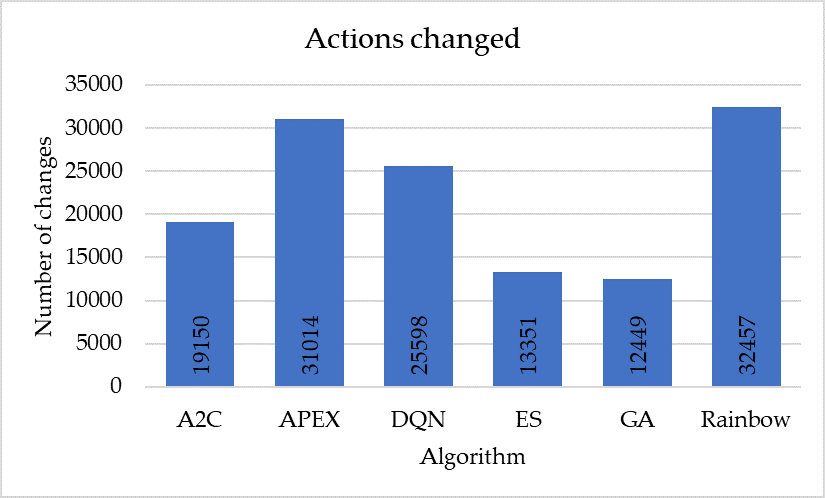
\includegraphics[scale=0.65]{source/images/eval/ac_changed}%
\caption[Number of actions changed]{The number of times an agent changed his action.}%
\label{fig:ac_changed}%
\end{figure}
The EA and GA algorithm primarily focused on two actions. Similarly, the A2C agent focused also on two actions; however, the action it did for around half of the game time was the \textit{noop} action, which does nothing. The other agents did not perform this action nearly as often, partially not at all.








